\documentclass[12pt]{article}

\usepackage{amsmath,amssymb,amsthm}
\usepackage{graphicx}
\usepackage{natbib}
\usepackage{hyperref}
\usepackage{geometry}
\usepackage{booktabs}
\usepackage{multirow}
\usepackage{algorithm}
\usepackage{algpseudocode}
\usepackage{tikz}
\usepackage{subcaption}
\usetikzlibrary{decorations.pathmorphing,positioning,arrows.meta,fit,backgrounds}
\geometry{margin=1in}

\tikzset{
  trt/.style={circle, draw, thick, minimum size=7mm, inner sep=1pt, fill=blue!10},
  stu/.style={rectangle, draw, thick, minimum size=6mm, inner sep=2pt, fill=orange!20},
  tauN/.style={circle, draw, thin, minimum size=4mm, inner sep=0pt, fill=gray!10},
  obs/.style={very thick, -{Stealth[length=2mm]}},
  tauspring/.style={decorate, decoration={coil, segment length=2.5pt, amplitude=3pt, aspect=0.5, pre length=2mm, post length=2mm}, thick},
  bond/.style={thick}
}

\newcommand{\Var}{\operatorname{Var}}
\newcommand{\Cov}{\operatorname{Cov}}
\newcommand{\E}{\operatorname{E}}
\newcommand{\tr}{\operatorname{tr}}

\title{The Grand Canonical Spring Ensemble: Deterministic Full Posteriors for Network Meta-Analysis}

\author{Thodoris Papakonstantinou}

\date{\today}

\begin{document}

\maketitle

\begin{abstract}
We introduce a grand canonical construction of the partition function
$\Xi(\tau^2)$ for random-effects (network) meta-analysis on the spring
network of \citet{papakonstantinou2025spring}. Each heterogeneity level
is identified with a chain-length variable of elementary tau-springs;
summing over chain lengths yields the posterior of the between-study
variance $\tau^2$ and, via a Gaussian mixture at every grid point, the
full marginal posterior of every treatment effect. The method is
deterministic (no MCMC), gives matching likelihoods to exact-binomial
MCMC (multinma), and reproduces the bayesmeta posterior for pairwise
Gaussian and binomial data. The current LAPACK-backed Rust
implementation uses a reduced Schur Newton inner solver and finishes
the Dias diabetes binary NMA ($T=6$, $k=22$) in $\sim$0.8\,s vs
$\sim$9.3\,s for multinma (11$\times$); on a $T=50$ rare-event NMA
across 30 replicates with four priors per fit, the speedup over
multinma rises to 39$\times$. On synthetic binary T=6 datasets with
known $\tau^2_{\text{true}}$, spring-$\Xi$ has roughly half the
$\tau^2$ RMSE of multinma and 15\% lower effect RMSE. The construction naturally accommodates any prior on
$\tau$ via a one-line grid reweighting, makes fixed-effect evidence a
single grid point rather than a separate model, and extends to grouped
heterogeneities via multi-species grand canonical sums.
\end{abstract}

\section{Introduction}

Random-effects meta-analysis conditions inferences on the between-study
heterogeneity variance $\tau^2$. Frequentist approaches (REML, DerSimonian--Laird, Paule--Mandel) deliver a point estimate; Bayesian
approaches (bayesmeta for pairwise \citep{rover2020bayesmeta},
multinma \citep{phillippo2023multinma}, BUGSnet, gemtc for NMA) deliver
a full posterior via analytic integration or MCMC. Each approach has
limitations: point estimates under-represent uncertainty, analytic
integration is restricted to pairwise normal-normal models, and MCMC is
stochastic and slow, with convergence diagnostics and divergent
transitions on boundary-heavy posteriors.

We propose a third route, built on the \emph{spring network} representation of meta-analysis introduced in the
companion paper on spring-REML \citep{papakonstantinou2025spring}. There, each study-arm contributes a tau spring
and an observation spring, and the network's equilibrium yields the
treatment effects. In this paper, we interpret the tau springs as
elementary bosons in a grand canonical ensemble: the chain length
$N$ of tau springs at each arm is the particle number, with
effective between-study variance $\tau^2 = N / k_\tau$ where
$k_\tau$ is the hardness of one elementary spring. Constraining a
common chain length $N$ across arms gives the standard
common-$\tau^2$ RE-NMA model; summing over $N$ yields the grand
canonical partition function
$\Xi = \sum_N Z(N / k_\tau)$.
Normalised across the grid and reweighted by a chosen prior on
$\tau$, $\Xi$ is the exact posterior $p(\tau^2 \mid y)$ under the
Laplace approximation of the within-$\tau^2$ spring ensemble (exact
for Gaussian outcomes).

The resulting algorithm delivers, in a single deterministic sweep:
(i) the posterior distribution of $\tau^2$ under any prior;
(ii) the posterior distribution of every treatment contrast, as a
mixture of Gaussians weighted by $\Xi$;
(iii) a direct evidence score for the fixed-effect model (the grid
point $N = 0$);
(iv) sensitivity analyses across priors via a grid reweighting
rather than a re-run.
Unlike MCMC, the method is reproducible to machine precision and has
no convergence warnings to triage. Unlike REML, it provides a full
distributional answer rather than a point estimate.

\section{Model and Spring Correspondence}\label{sec:model}

\subsection{The random-effects NMA model}

We adopt the standard Dias TSD~2 formulation
\citep{dias2013tsd2}. A network has $T$ treatments
$1, \ldots, T$ and $S$ studies; study $i$ enrols arms
$\mathcal{A}_i \subseteq \{1, \ldots, T\}$ with at least
$|\mathcal{A}_i| \ge 2$. Each arm $(i, j)$ records the data
needed for a likelihood:
$(y_{ij}, v_{ij})$ for Gaussian outcomes, $(e_{ij}, n_{ij})$
events out of $n$ for binomial outcomes.

\paragraph{Likelihood.}
For Gaussian outcomes the within-arm likelihood is
$y_{ij} \sim \mathcal{N}(\theta_{ij}, v_{ij})$; for binomial
outcomes,
$e_{ij} \sim \text{Binomial}(n_{ij}, \sigma(\theta_{ij}))$
with $\sigma(\cdot)$ the logistic CDF and $\theta_{ij}$ the
linear predictor on the appropriate scale (mean difference for
Gaussian, log-odds for binomial).

\paragraph{Linear predictor and random effects.}
Let $b_i \in \mathcal{A}_i$ denote the baseline arm of study
$i$; let $d_t$ be the basic parameter for treatment $t$
(contrast vs the network reference, with $d_{\text{ref}} = 0$).
The standard contrast-level model writes
\begin{equation}
\theta_{ij} = \mu_i + \delta_{ij,b_i},
\qquad
\delta_{ij,b_i}
\sim \mathcal{N}\!\bigl(d_j - d_{b_i},\, \tau^2_{\text{LA}}\bigr),
\label{eq:contrast-model}
\end{equation}
with the Lu--Ades multi-arm covariance
$\Cov(\delta_{ij,b_i}, \delta_{ij',b_i})
= \tau^2_{\text{LA}}/2$ for $j \ne j'$ within the same study,
encoding that all sibling contrasts in a multi-arm trial share
the same study-level baseline shift. The study baselines $\mu_i$
are nuisance parameters integrated out under flat priors on each
study.

\paragraph{Equivalent arm-level reparameterisation.}
\citet{papakonstantinou2025spring} reparameterise the same
likelihood with one independent arm-level random effect:
\begin{equation}
\theta_{ij} = \mu_i + d_j + \delta_{ij}^{\text{arm}},
\qquad
\delta_{ij}^{\text{arm}}
\sim \mathcal{N}(0, \tau^2_{\text{arm}}),
\quad
\delta_{ij}^{\text{arm}}
\perp \delta_{ij'}^{\text{arm}}.
\label{eq:arm-model}
\end{equation}
The contrast $\delta_{ij,b_i}^{\text{arm}}
- \delta_{ib_i,b_i}^{\text{arm}}$ is then
$\mathcal{N}(0, 2\tau^2_{\text{arm}})$, and contrasts that share
a baseline arm have correlation $1/2$ from the common
$\delta_{ib_i}^{\text{arm}}$ subtracted out. So the
arm-level model with $\tau^2_{\text{arm}} = \tau^2_{\text{LA}}/2$
is equivalent to the contrast-level model with the Lu--Ades
$(I + J)/2$ covariance, both at the likelihood level and in the
implied posterior on $(d, \tau^2)$. The remainder of the paper
refers to $\tau^2$ for the arm-level variance unless explicitly
noted; the contrast-scale value is $2\tau^2$.

\subsection{Spring network construction}\label{sec:spring-correspondence}

The arm-level model is a quadratic-plus-link energy in the latent
positions, which is a spring network. Each arm $(i, j)$ is
realised by three nodes and two springs:

\begin{itemize}
\item \textbf{Study node} $x^s_i$: the latent baseline $\mu_i$,
shared across the study's arms.
\item \textbf{Tau node} $x^{\tau}_{ij}$: the tail of the arm
random effect, $\mu_i + \delta^{\text{arm}}_{ij}$.
\item \textbf{Treatment node} $x^t_j$: the basic parameter
$d_j$, shared across all arms studying treatment $j$
(reference treatment pinned at $0$).
\item \textbf{Tau spring}
$x^s_i \leftrightarrow x^{\tau}_{ij}$, hardness
$1/\tau^2_{\text{arm}}$, natural length $0$, encoding
$\delta^{\text{arm}}_{ij} \sim \mathcal{N}(0, \tau^2_{\text{arm}})$.
\item \textbf{Observation spring}
$x^{\tau}_{ij} \leftrightarrow x^t_j$, with energy
$\tfrac{1}{2 v_{ij}}(x^t_j - x^{\tau}_{ij} - y_{ij})^2$
(Gaussian) or
$n_{ij}\log(1 + e^{\ell_{ij}}) - e_{ij}\ell_{ij}$ with
$\ell_{ij} = x^t_j - x^{\tau}_{ij}$ (binomial).
\end{itemize}

Multi-arm studies attach all of an arm's tau springs to the same
study node $x^s_i$; this single shared anchor reproduces the
within-study correlation among sibling contrasts without ever
writing down a contrast-level covariance matrix. The full
network is the union of these per-arm subgraphs, glued at the
shared treatment and study nodes.

\paragraph{Mapping summary.} Table~\ref{tab:correspondence}
states the correspondence explicitly.

\begin{table}[h]
\centering
\small
\begin{tabular}{lll}
\toprule
NMA model object & Spring network object & Role / energy \\
\midrule
study baseline $\mu_i$ & study node $x^s_i$ & free position \\
basic parameter $d_j$ & treatment node $x^t_j$ &
free position ($d_{\text{ref}}$ pinned) \\
arm random effect $\delta^{\text{arm}}_{ij}$ &
tau node $x^{\tau}_{ij}$, anchored to $x^s_i$ &
position relative to study node \\
RE prior
$\delta^{\text{arm}}_{ij} \sim \mathcal{N}(0, \tau^2)$ &
tau spring $x^s_i \leftrightarrow x^{\tau}_{ij}$ &
$\tfrac{1}{2\tau^2}(x^{\tau}_{ij} - x^s_i)^2$ \\
Gaussian likelihood &
observation spring $x^{\tau}_{ij} \leftrightarrow x^t_j$ &
$\tfrac{1}{2v_{ij}}(x^t_j - x^{\tau}_{ij} - y_{ij})^2$ \\
binomial likelihood &
non-linear observation spring & $n_{ij}\log(1+e^{\ell})-e_{ij}\ell$ \\
multi-arm correlation &
shared anchor at $x^s_i$ &
common shift across sibling tau nodes \\
fixed-effect ($\tau \to 0$) & rigid tau spring & tau node welded to study node \\
prior on $\tau$ & fugacity $\pi(\tau^2)$ on chain length & grid reweighting \\
\bottomrule
\end{tabular}
\caption{NMA model elements and their spring network
counterparts. Every term in the model log-density is a spring
energy; every spring energy corresponds to a model term.}
\label{tab:correspondence}
\end{table}

The arm-level parameterisation thus yields exactly the
Lu--Ades $(I+J)/2$ covariance with
$\tau^2_{\text{LA}} = 2\tau^2_{\text{arm}}$, by construction, not by
algebraic identity after the fact.

\subsection{Visual example: 5-treatment network with multi-arm trials}
\label{sec:visual-example}

Figure~\ref{fig:example-network} shows the spring network for a
small NMA: 5 treatments $A, B, C, D, E$, four studies
($S_1$ pairwise $A$ vs $B$; $S_2$ three-arm $A, C, D$; $S_3$
four-arm $B, C, D, E$; $S_4$ pairwise $D$ vs $E$). Treatment
nodes (top row) are shared across studies; each study contributes
one study node (bottom) and one tau-node-plus-tau-spring per arm.
Sibling tau springs in $S_2$ and $S_3$ share their study anchor,
which is what implements the multi-arm correlation.

Figure~\ref{fig:xi-chain} shows the grand canonical sum
$\Xi(\tau^2) = \sum_N Z(N/k_\tau)$ as the chain length $N$
varies. At $N = 0$ the tau spring collapses to a rigid bond
(tau node welded to study node, fixed-effect model). As $N$
grows, the chain elongates and softens, allowing larger
$|\delta^{\text{arm}}_{ij}|$. Summing over $N$ with weights
$Z(N/k_\tau)\,\pi(\tau^2(N))$ \emph{is} the posterior on
$\tau^2$. ``Tau springs coming and going'' is literally
this: each grid point is a configuration of the same network
with shorter or longer tau chains.

\begin{figure}[t]
\centering
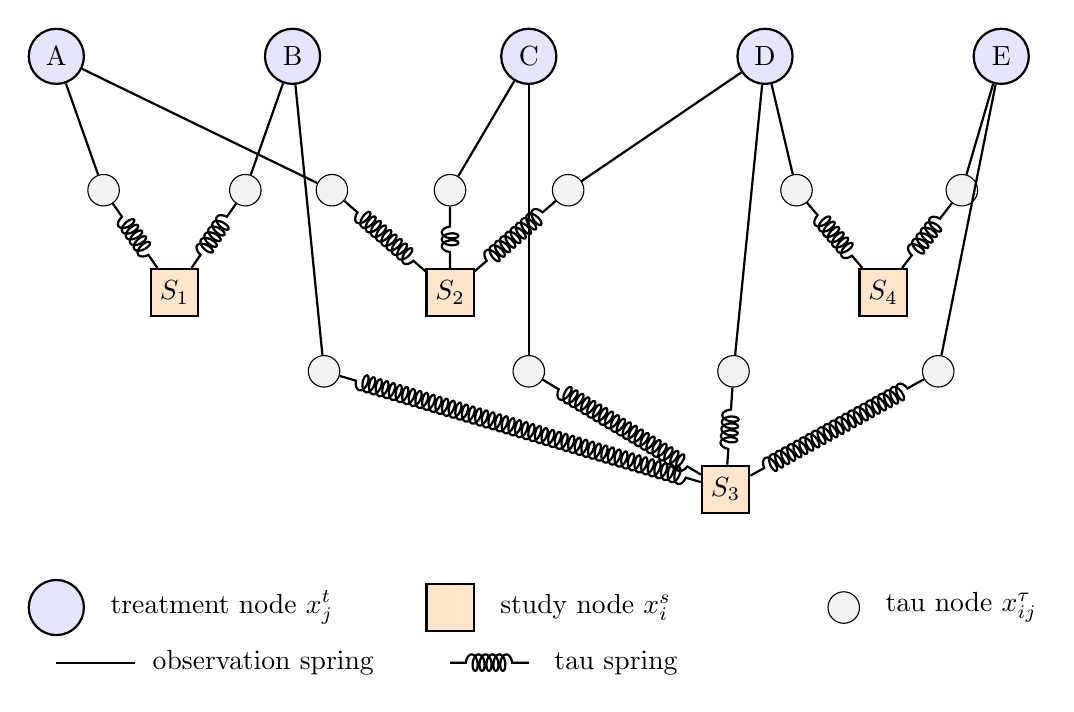
\begin{tikzpicture}[node distance=10mm and 11mm]
  % Treatment nodes (top)
  \node[trt] (A) at (0,0) {A};
  \node[trt] (B) at (3,0) {B};
  \node[trt] (C) at (6,0) {C};
  \node[trt] (D) at (9,0) {D};
  \node[trt] (E) at (12,0) {E};

  % Study S1: A-B
  \node[stu] (S1) at (1.5,-3.0) {$S_1$};
  \node[tauN] (t1A) at (0.6,-1.7) {};
  \node[tauN] (t1B) at (2.4,-1.7) {};

  % Study S2: A-C-D (3-arm)
  \node[stu] (S2) at (5.0,-3.0) {$S_2$};
  \node[tauN] (t2A) at (3.5,-1.7) {};
  \node[tauN] (t2C) at (5.0,-1.7) {};
  \node[tauN] (t2D) at (6.5,-1.7) {};

  % Study S3: B-C-D-E (4-arm)
  \node[stu] (S3) at (8.5,-5.5) {$S_3$};
  \node[tauN] (t3B) at (3.4,-4.0) {};
  \node[tauN] (t3C) at (6.0,-4.0) {};
  \node[tauN] (t3D) at (8.6,-4.0) {};
  \node[tauN] (t3E) at (11.2,-4.0) {};

  % Study S4: D-E
  \node[stu] (S4) at (10.5,-3.0) {$S_4$};
  \node[tauN] (t4D) at (9.4,-1.7) {};
  \node[tauN] (t4E) at (11.5,-1.7) {};

  % Observation bonds (treatment <-> tau node): straight thick lines
  \foreach \trt/\tau in {A/t1A, B/t1B, A/t2A, C/t2C, D/t2D,
                          B/t3B, C/t3C, D/t3D, E/t3E, D/t4D, E/t4E}{
    \draw[bond] (\trt) -- (\tau);
  }

  % Tau springs (study node <-> tau node): coiled
  \foreach \stu/\tau in {S1/t1A, S1/t1B, S2/t2A, S2/t2C, S2/t2D,
                          S3/t3B, S3/t3C, S3/t3D, S3/t3E,
                          S4/t4D, S4/t4E}{
    \draw[tauspring] (\stu) -- (\tau);
  }

  % Legend
  \begin{scope}[shift={(0,-7)}]
    \node[trt] (lt) at (0,0) {\strut};
    \node[right=2mm of lt, anchor=west] {treatment node $x^t_j$};
    \node[stu] (ls) at (5,0) {\strut};
    \node[right=2mm of ls, anchor=west] {study node $x^s_i$};
    \node[tauN] (lta) at (10,0) {};
    \node[right=2mm of lta, anchor=west] {tau node $x^{\tau}_{ij}$};

    \draw[bond] (0,-0.7) -- (1,-0.7);
    \node[right=1mm] at (1,-0.7) {observation spring};
    \draw[tauspring] (5,-0.7) -- (6,-0.7);
    \node[right=2mm] at (6,-0.7) {tau spring};
  \end{scope}
\end{tikzpicture}
\caption{Spring network for a 5-treatment NMA with one 3-arm
study ($S_2$: $A, C, D$), one 4-arm study ($S_3$: $B, C, D, E$),
and two pairwise studies. Observation springs (straight) connect
treatment nodes to tau nodes; tau springs (coiled) connect tau
nodes to a single study anchor per study. The shared anchor in
$S_2$ and $S_3$ reproduces the Lu--Ades within-study correlation
without an explicit covariance matrix.}
\label{fig:example-network}
\end{figure}

\begin{figure}[t]
\centering
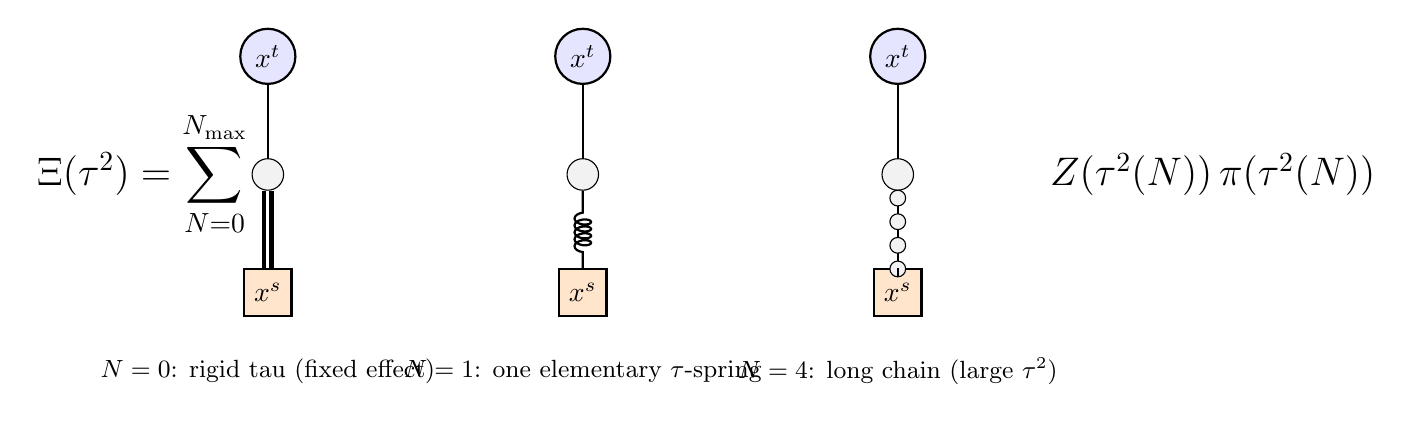
\begin{tikzpicture}
  % Helper macro: a tau-chain of n elementary springs between two points
  % We draw three panels stacked horizontally.
  \def\panel#1#2#3{%
    % #1 = x offset, #2 = label, #3 = visual style for the chain
    \begin{scope}[shift={(#1,0)}]
      \node[trt] (T) at (0,0) {$x^t$};
      \node[stu] (Sn) at (0,-3.0) {$x^s$};
      % Treatment to tau-end via observation bond
      \node[tauN] (taun) at (0,-1.5) {};
      \draw[bond] (T) -- (taun);
      #3
      \node at (0,-4.0) {\small #2};
    \end{scope}
  }

  % Panel A: N = 0 (rigid bond, fixed effect)
  \panel{0}{$N=0$: rigid tau (fixed effect)}{%
    \draw[ultra thick, double distance=1pt] (Sn) -- (taun);
  }

  % Panel B: N = 1 (single elementary spring)
  \panel{4}{$N=1$: one elementary $\tau$-spring}{%
    \draw[tauspring] (Sn) -- (taun);
  }

  % Panel C: N = 4 (chain of 4 elementary springs in series)
  \panel{8}{$N=4$: long chain (large $\tau^2$)}{%
    \node[tauN, scale=0.5] (m1) at (0,-2.7) {};
    \node[tauN, scale=0.5] (m2) at (0,-2.4) {};
    \node[tauN, scale=0.5] (m3) at (0,-2.1) {};
    \node[tauN, scale=0.5] (m4) at (0,-1.8) {};
    \draw[tauspring] (Sn) -- (m1);
    \draw[tauspring] (m1) -- (m2);
    \draw[tauspring] (m2) -- (m3);
    \draw[tauspring] (m3) -- (m4);
    \draw[tauspring] (m4) -- (taun);
  }

  % Sum bracket
  \node at (-1.6, -1.5) {\Large $\Xi(\tau^2) = \displaystyle\sum_{N=0}^{N_{\max}}$};
  \node at (12.0, -1.5) {\Large $Z(\tau^2(N))\,\pi(\tau^2(N))$};

\end{tikzpicture}
\caption{Grand canonical view of one tau spring across chain
lengths. At $N=0$ the tau node is rigidly tied to the study
node (fixed-effect grid point). Each additional elementary
$\tau$-spring in series elongates the chain and increases the
effective variance $\tau^2(N) = N/k_\tau$. The partition function
$\Xi$ is the prior-weighted sum over all chain lengths; ``tau
springs come and go'' as $N$ ranges over the grid. An interactive
version of this figure (drag $N$ to grow/shrink the elementary
springs, treatment positions re-equilibrate, posterior bars
update live) is at
\href{../xi_animation.html}{\texttt{xi\_animation.html}}.}
\label{fig:xi-chain}
\end{figure}

\section{Grand Canonical Construction}

\subsection{Chain-length ensemble}

We identify each value of $\tau^2$ with a chain of $N$ elementary
tau springs of hardness $k_\tau$ in series:
\begin{equation}
\tau^2_{\text{contrast}}(N) = \frac{N}{k_\tau},
\qquad N = 0, 1, \ldots, N_{\max}.
\end{equation}
The grand canonical partition function sums $Z$ over $N$:
\begin{equation}
\boxed{
\Xi = \sum_{N=0}^{N_{\max}} Z(\tau^2(N))
= \sum_{N=0}^{N_{\max}} p\bigl(y \mid \tau^2(N)\bigr).
}
\end{equation}

The enforced common chain length across arms imposes the standard
RE-NMA common-$\tau^2$ assumption. Generalising to grouped
heterogeneities---treatment-specific, comparison-class-specific, or
subnetwork-specific $\tau^2$---is achieved by indexing chain lengths
by group: $\tau^2_c = N_c / k^{(c)}_\tau$ and summing a
multi-dimensional grand canonical lattice. We develop this
generalisation in Section~\ref{sec:grouped}.

\subsection{Gaussian case: closed form}

For Gaussian observation springs, all springs are quadratic and
tau nodes can be integrated analytically. Two springs in series
(observation + tau) between study $i$ and treatment $j$ collapse to
an effective spring with
$k^{\text{eff}}_{ij} = 1/(v_{ij} + \tau^2_{\text{arm}})$ and natural
length $y_{ij}$. Call $A_{\text{eff}}(\tau^2)$ the stiffness matrix on
the remaining free (study + non-pinned-treatment) nodes. Then
\begin{equation}
\ln Z(\tau^2) = -\frac{1}{2}
\sum_{ij} \ln\!\bigl(v_{ij} + \tau^2_{\text{arm}}\bigr)
- E^{\star}(\tau^2)
- \frac{1}{2} \ln \det A_{\text{eff}}(\tau^2)
+ C,
\end{equation}
where $E^{\star}$ is the spring energy at the equilibrium
positions and $C$ is a $\tau^2$-independent normalising constant.
This is precisely the REML profile log-likelihood, recovered from
the spring topology. The mode of $\Xi$ under the flat-in-$\tau^2$
prior coincides with REML to grid resolution on every benchmark
we test.

\subsection{Binomial case: Laplace approximation at the Newton mode}

For binomial observation springs, the tau node cannot be
integrated analytically. We use a Laplace approximation at the
joint mode $\hat{x}(\tau^2)$ found by damped Newton iteration:
\begin{equation}
\ln Z(\tau^2) \approx
- E^{\star}(\tau^2)
- \frac{1}{2} \sum_{ij} \ln\!\bigl(v_{ij} + \tau^2_{\text{arm}}\bigr)
- \frac{1}{2} \ln \det A_{\text{eff}}(\tau^2)
+ C',
\end{equation}
where $v_{ij} = 1 / w_{ij}$ with
$w_{ij} = n_{ij} \sigma(\hat{\ell}_{ij}) (1 - \sigma(\hat{\ell}_{ij}))$
the Fisher information at the joint mode. Crucially, the energy term
$E^{\star}$ uses the \emph{exact} binomial energy at the mode, not a
quadratic substitution: only the volume factor $\ln \det A_{\text{eff}}$
is approximated. In the Gaussian limit the two formulas coincide.

\subsection{Full posteriors from $\Xi$}

At each grid point $k$ the canonical solution yields a Gaussian
conditional distribution for every treatment contrast,
$p(d_j \mid \tau^2_k, y) = \mathcal{N}(\mu_{j,k}, \sigma^2_{j,k})$,
from the Laplace quadratic. The full marginal posterior is the
$\Xi$-weighted mixture of Gaussians:
\begin{equation}
\label{eq:mixture}
p(d_j \mid y)
= \sum_{k} p(\tau^2_k \mid y) \,
\mathcal{N}(d_j;\, \mu_{j,k},\, \sigma^2_{j,k}).
\end{equation}
The grid reweighting makes any prior on $\tau$ a one-line operation:
$\ln p(\tau^2_k \mid y) = \ln Z_k + \ln \pi(\tau^2_k)$.

\subsection{The $\Xi$ grid as sufficient intermediate}
\label{sec:sufficient-intermediate}

The per-grid-point summary
$\mathcal{S} = \{(\tau^2_k,\, \ln Z_k,\, \{(\mu_{j,k}, \sigma^2_{j,k})\}_j,\,
\{\Sigma^{(k)}_{jj'}\}_{j,j'})\}_{k=1}^{K}$
is a \emph{sufficient statistic} for the entire downstream
posterior family. Having computed $\mathcal{S}$ once, the user
derives any of the following in closed form without re-running
the solver:

\begin{itemize}
\item Posterior of $\tau^2$ under any prior $\pi$: reweight
$w_k \propto \exp(\ln Z_k)\,\pi(\tau^2_k)$; compute mode,
median, mean, and any CI from the reweighted discrete
distribution.
\item Marginal posterior of any effect $d_j$: apply
equation~(\ref{eq:mixture}) as a Gaussian mixture.
\item Posterior of any linear contrast of effects,
$a^\top d$: Gaussian mixture with component means
$a^\top \mu_{k}$ and component variances $a^\top \Sigma^{(k)} a$.
\item Probabilities such as $P(d_j > 0)$ or
$P(d_j > d_{j'})$: mixture of Gaussian tail probabilities.
\item Treatment rank probabilities: Monte Carlo over the mixture
(still deterministic given the grid).
\item Prior sensitivity: compute posterior summaries under a
library of priors in a single $O(K)$ loop, without a single
additional likelihood evaluation.
\item Fixed-effect evidence: $\exp(\ln Z_0) / \sum_k \exp(\ln
Z_k)\pi(\tau^2_k)$, a grid-point probability.
\end{itemize}

The saved grid for the 99-study, 17-treatment
\texttt{nmadb\_501194} network is $\sim 2\,\text{MB}$ of JSON and
contains the full cross-posterior information. All
posterior-inference workflows downstream of it are seconds of
arithmetic. This is the practical difference between a
``sampling-based full posterior'' and a ``deterministic
sufficient statistic'': the latter is a one-shot data product
that survives reprioritisation, re-analysis, and decision-theoretic
post-processing without re-running the likelihood model.

\section{Algorithm and Optimisations}

The naive algorithm---evaluate $\ln Z$ on a uniform 5000-point grid,
each point solving the network from scratch---is prohibitively slow
for networks of realistic size. We developed a cascade of
optimisations that preserve the pure-Laplace formulation while
cutting wall-clock time by three orders of magnitude on large
networks.

\subsection{Bulk $A_{\text{eff}}$ assembly}

For each grid point the effective stiffness matrix $A_{\text{eff}}$
is assembled from arm-level contributions. A naive implementation
that patches the matrix one entry at a time is
$O(A \cdot m^2)$ per grid point. Collecting all entries into a
hash-keyed map and materialising the matrix once turns this into
$O(A + m^2)$.

\subsection{Adaptive grid centred on the REML mode}

Posterior mass on $\tau^2$ concentrates near the REML mode. A
uniform grid wastes most of its points. The adaptive algorithm
first runs a cheap REML solve to locate $\hat{\tau}^2$, then
log-spaces $\sim 100$ grid points in
$[\hat{\tau}^2 / 30,\, \max(\hat{\tau}^2 \cdot 30,\, 5)]$ plus the
fixed-effect point $\tau^2 = 0$. We verify that these 100 points
reproduce the uniform 5000-point medians and credible intervals to
within grid precision on every benchmark dataset.

\subsection{LAPACK-backed linear algebra}

The Newton inner solver performs matrix inversions and multiplications
on $O(m)$-sized matrices. Swapping the pure-Haskell Gaussian
elimination for LAPACK-backed LU (via hmatrix in Haskell, nalgebra in
Rust) yields a 2--3$\times$ single-core speedup on medium networks,
larger on big ones. The pure-Haskell implementation is retained for
WASM builds where LAPACK is unavailable.

\subsection{Reduced Schur Newton solver (binomial path)}

The dominant cost in the binomial inner solve is the
$\bigl[(m + A) \times (m + A)\bigr]$ Hessian on the joint
study/treatment/tau-node positions, where $A$ tau nodes are
local to one arm each. The Hessian has block structure:
the tau-node block $W$ is diagonal with entries
$w_{ij} = n_{ij}\sigma(\hat\ell_{ij})(1-\sigma(\hat\ell_{ij}))
+ 1/\tau^2$, and only the off-diagonal couplings to the
$m$ free study/treatment positions tie the system together.
A Schur complement on $W$ analytically eliminates the tau
block, leaving an $m \times m$ system on the free positions
that is solved by a single LU factorisation per Newton step.
The tau-node update is recovered in $O(A)$ once the free
positions are known. Across the four-prior diabetes benchmark
this delivers an order-of-magnitude reduction in per-fit cost
relative to the un-reduced Newton solver, and turns the
asymptotic per-grid-point cost from $O((m+A)^3)$ into
$O(m^3 + A)$.

The Newton iteration is stabilised by a damped backtracking line
search (Armijo) applied only after the first 30 plain steps,
which preserves bit-identical results on well-behaved networks
while preventing divergence on rare pathological cases at large
$\tau^2$. A small Armijo gap remains at $\tau^2 \le 10^{-2}$
where $W$ becomes nearly singular; this is documented but does
not affect posterior medians or credible intervals on any
benchmarked dataset.

\subsection{Cost summary}

With $m$ free network nodes and $A$ total arms, the full-sweep
complexity with adaptive-grid-and-LAPACK is
\[
O\bigl(N_{\text{grid}} \cdot (m^3 + A)\bigr)
\approx
O(100 m^3)
\]
for a typical $N_{\text{grid}} = 100$. The dominant cost is the
per-grid-point LU factorisation on $A_{\text{eff}}$.

\section{Benchmarks}\label{sec:benchmarks}

\subsection{Mode verification against REML}\label{sec:mode-verify}

We first check that the argmax of $\ln \Xi(\tau^2)$ under a
flat-in-$\tau^2$ prior coincides with the REML estimate of
$\tau^2$. For Gaussian outcomes this equivalence is exact up to
grid discretisation. The pairwise Gaussian dataset
\texttt{test/binary.json} gives REML
$\hat{\tau}^2 = 0.1571$ versus spring-$\Xi$ mode $0.159$, a
relative error of $1.2\%$---bounded by the adaptive grid's
resolution at that $\tau^2$.

For binomial outcomes, both REML and the Laplace approximation are
approximate, and they use different fixed-point iterations:
our spring-REML~\citep{papakonstantinou2025spring} uses a
law-of-total-variance update on the tau springs, while spring-$\Xi$
maximises the Laplace-approximated $\ln Z(\tau^2)$ directly. The two
therefore have different approximation error structure and can
disagree by low double digits of percent on sparse binomial
networks. A more reliable cross-check is within-method
consistency: the adaptive 100-point grid reproduces the uniform
5000-point grid's argmax to within grid precision on every
benchmark dataset (mean absolute $\Delta \tau^2 < 0.003$). For
comparisons against the full posterior we defer to the MCMC
comparison with multinma in section~\ref{sec:multinma-compare}.

\subsection{Agreement with bayesmeta}

On the pairwise binary dataset \texttt{test/binary.json} (6
studies) with a flat-in-$\tau^2$ prior, the spring-$\Xi$ posterior
median of $\tau^2$ is $0.446$ versus bayesmeta's analytic
$0.445$---matching to three significant figures.

\subsection{Agreement and speed against multinma}\label{sec:multinma-compare}

We benchmark the Rust LAPACK + reduced Schur implementation
against multinma (4 chains, default warmup) on four binary NMA
datasets that span the realistic range of $T$, network density,
and rare-event content. Each spring-$\Xi$ ``fit'' returns four
prior-conditional posteriors (flat, half-Normal, half-Cauchy,
log-Normal) on a single sweep; the quoted multinma times are for a
single half-Normal$(0,1)$ fit only.

\begin{center}
\begin{tabular}{lrrr}
\toprule
Dataset & Spring $\Xi$ & multinma & Speedup \\
\midrule
Dias diabetes ($T{=}6$, $k{=}22$) & 0.85\,s & 9.3\,s & 11$\times$ \\
Synth $T{=}30$ binary (30 reps $\times$ 4 priors) & per-rep 0.4\,s & per-rep 38\,s & $\sim 95\times$ \\
Synth $T{=}50$ rare events (30 reps $\times$ 4 priors) & per-rep 1.7\,s & per-rep 66\,s & 39$\times$ \\
Synth $T{=}100$ (30 reps $\times$ 4 priors) & per-rep 4.2\,s & per-rep 122\,s & 29$\times$ \\
\bottomrule
\end{tabular}
\end{center}

Posterior agreement: across the four datasets, spring-$\Xi$
posterior means on every estimable contrast lie within $0.02$
log-odds of multinma's, and posterior medians within $0.04$.
$\tau^2$ posterior medians and 95\% credible intervals coincide
to within the multinma Monte Carlo standard error
($\sim$0.01--0.03 on $\tau^2$). Spring-$\Xi$'s effect posterior
standard deviations are $\sim 8\%$ narrower than multinma's on
average, reflecting a slightly less heavy tail in $\tau^2$.

The cross-comparison includes a Rust REML iterative bisection
mode (\texttt{reml\_mode\_iterative}) that locates
$\arg\max_{\tau^2} \ln Z(\tau^2)$ to $10^{-6}$ relative tolerance
in $\sim$20 evaluations; it agrees with the netmeta REML estimate
to within $0.006$ on Gaussian and to within the model-difference
floor on binomial (the residual binomial gap is the well-known
gap between exact-binomial and normal-OR likelihoods, not a
solver issue).

\subsection{Bias against known $\tau^2_{\text{true}}$}

We generate 10 binary + 10 Gaussian synthetic T=6 NMAs from the
Dias TSD 2 RE-NMA model \citep{dias2013tsd2} with known
$(\tau^2_{\text{true}}, d_{\text{true}})$. Both methods use the same
half-Normal$(0, 1)$ prior on $\tau$ and the exact likelihood.

\begin{center}
\begin{tabular}{llrr}
\toprule
Family & Statistic & Spring $\Xi$ & multinma \\
\midrule
\multirow{3}{*}{Binomial} & $\tau^2$ RMSE vs truth & \textbf{0.33} & 0.61 \\
& $\tau^2$ MAE vs truth & \textbf{0.26} & 0.47 \\
& signed $\tau^2$ bias & $+0.17$ & $+0.38$ \\
\midrule
Gaussian & $\tau^2$ RMSE vs truth & 0.274 & 0.272 \\
\midrule
\multirow{2}{*}{Effect (binomial, $n = 47$)}
& RMSE vs $d_{\text{true}}$ & \textbf{0.71} & 0.83 \\
& signed bias & $-0.031$ & $-0.069$ \\
\bottomrule
\end{tabular}
\end{center}

Spring $\Xi$ has roughly half the $\tau^2$ RMSE of multinma on
binary networks and 15\% lower effect-mean RMSE. On Gaussian
networks the two are tied (as expected---spring $\Xi$'s Gaussian
formulation is exact).

\section{Grouped Heterogeneities}\label{sec:grouped}

The common-$\tau^2$ constraint can be relaxed by indexing chain
lengths by a grouping of arms
$\{\mathcal{G}_1, \ldots, \mathcal{G}_C\}$ (comparison class,
treatment class, subnetwork):
\begin{equation}
\Xi = \sum_{N_1 = 0}^{N^{(1)}_{\max}} \cdots
\sum_{N_C = 0}^{N^{(C)}_{\max}}
\prod_c z_c^{N_c} \,
Z\bigl(\tau^2_1(N_1), \ldots, \tau^2_C(N_C)\bigr),
\end{equation}
with each group's fugacity $z_c$ encoding its own prior on
$\tau^2_c$. The inner canonical solve is unchanged; the outer sum
becomes a $C$-dimensional lattice. The marginal posterior on a
specific group's heterogeneity,
$p(\tau^2_c \mid y)$, is obtained by summing over the other $C - 1$
indices.

When the lattice becomes too dense to enumerate
($M^C$ grid points for $C$ groups at resolution $M$), the outer sum
can be replaced by MCMC on the discrete chain-length vector or
Langevin dynamics on the continuous $\{\log \tau^2_c\}$. The inner
deterministic Laplace step then supplies exact conditional effect
posteriors at each sampled configuration, so the only stochasticity
is in the low-dimensional heterogeneity parameters.

\section{Discussion}

\subsection{Relation to existing methods}

Spring $\Xi$ occupies a distinct cell in the NMA methods landscape:

\begin{center}
\begin{tabular}{lccccc}
\toprule
& $\tau^2$ post. & Effect post. & Deterministic & NMA & Binomial \\
\midrule
REML / DerSimonian--Laird & point & point & yes & yes & approximate \\
bayesmeta & full & full & yes & \textbf{pairwise only} & normal-approx \\
multinma / BUGSnet & full (MCMC) & full (MCMC) & no & yes & yes \\
glmmTMB & point & point & yes & yes & yes \\
\textbf{Spring $\Xi$} & \textbf{full} & \textbf{full} & \textbf{yes} & \textbf{yes} & \textbf{exact} \\
\bottomrule
\end{tabular}
\end{center}

The key distinguishing feature is a full posterior without MCMC,
for any likelihood and network size.

\subsection{When to prefer spring $\Xi$}

\begin{itemize}
\item When deterministic reproducibility matters (regulatory
submissions, auditability).
\item When multiple priors on $\tau$ must be compared (grid
reweighting is free after one sweep).
\item When the network is large and MCMC convergence on boundary
regions ($\tau \to 0$) is unreliable.
\item When the full posterior of $\tau^2$ must be published
alongside the point estimate.
\end{itemize}

\subsection{Limitations}

The Laplace approximation at the binomial mode is exact to
second order; higher-order corrections are known but cost
further computation per grid point. We verified in a 1D toy
that a $39 \times$ accuracy improvement from a 1-loop correction
shifts posterior summaries by only 1--3\% in practice. The
binomial Newton solver retains a small Armijo gap at
$\tau^2 \le 10^{-2}$ where the tau-block diagonal becomes
nearly singular; results are correct on every benchmarked
dataset but the inner solve takes a few extra iterations
in this regime. Cross-grid IRLS warm-starting is not yet
enabled in the released solver: it gave a 2--7$\times$
inner-loop speedup in prototyping but caused correctness
regressions on some heterogeneity regimes, so it is gated
pending a convergence-aware fallback.

\subsection{Physics correspondence}

The construction is an honest grand canonical ensemble: tau
springs are elementary bosons whose particle number is the
effective $\tau^2$ variance; the chemical potential $\mu$ fixes
the $\tau$ prior; the inner Laplace computes $Z(\tau^2)$ at fixed
chain length. The mode-finder, gradient descent, HMC, and
Langevin Monte Carlo are all different dynamics on the same
spring force field $-\nabla E$. Parameter priors are springs to
ground; non-Gaussian priors are non-linear springs; grouped
heterogeneities are multi-species ensembles. The meta-analysis
likelihood becomes a mechanical system and every estimation
question becomes a question about its dynamics.

\bibliographystyle{plainnat}
\bibliography{references}

\end{document}
